\chapter{Mudança de suporte e curvas de teor e tonelagem}


\section{Mudança de suporte}

Após realizada a krigagem dos dados é interessante comparar o efeito da suavização da krigagem. Esta possui duas forças envolvendo a estimativa em um local, uma relacionada com a interpolação dos dados e outra com a suavização dada pela tomada de valores médios. 

A fim de comparar as estatísticas estimadas com as amostras podemos tranformar a primeira em um suporte pontual. Logo a diferença entre os seus valores será apenas o efeito da suavização. Como demonstrado no capítulo 1 na figura \eqref{Efeito_Suporte2}, a variância do valor médio tende a estreitar com o aumento do suporte utilizado. Para comparar os histogramas precisamos então realizar um "esticamento" da distribuição.


\begin{figure}[H]
	\centering
	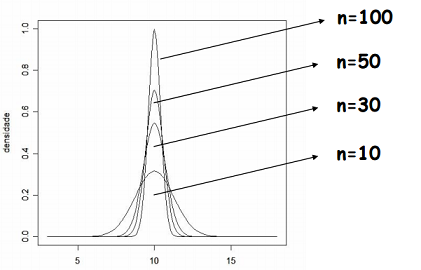
\includegraphics[scale=1.0]{EfeitoSuporte.png}	
	\caption{Figura demonstrando o efeito de suporte para um número crescente de amostras. O aumento do número de amostras tende a concentrar a  função de densidade de probabilidade entorno do valor médio }
	\label{Efeito_Suporte2}
\end{figure} 

Duas premissas devem ser tomadas antes de se realizar a correção de suporte. A primeira é de que o valor médio permanece constante. A segunda é que a variância da distribuição é corrigida por um fator "f". Esse fator f pode ser descrito pela equação \eqref{suporte1}

\begin{equation}\label{suporte1}
	f= \frac{\sigma^2_{0} - \bar{\gamma}(V,V)}{\sigma^2_{0}}
\end{equation}

Em que $\bar{\gamma}(V,V)$ é o valor de variograma médio dentro do suporte V a ser corrigido e $\sigma^2_{0}$ é o valor de variância à priori dos dados. 

\subsection{Correção afim}

Uma das formas mais simples de se realizar a correção de suporte é mudando a distribuição de probabilidades por um fator linear. Essa também é chamada de "affine correction" ou correção afim, em que o valor da média da distribuição é mantida constante mas a variância sofre extensões de igual valor dado pela equação  \eqref{affine}

\begin{equation}\label{affine}
q'= \sqrt{f}*(q-m) + m
\end{equation}

em que q é o quartil a ser transformado, m o valor médio e f o fator de correção demonstrado na seção anterior. Essa transformação linear proposta pelo método produz em alguns casos valores anômalos principalmente nas terminações das distribuições que apresentam comportamento muito mais assintótico que os valores centrais. 

\subsection{Transformação lognormal indireta}

De forma a corrigir o comportamento das distribuições de forma mais assintótica nas terminações da distribuição, o método de transformação lognormal indireta propõe uma resoulção não linear para o problema, tal que cada quartil pode ser dado pela equação \eqref{affinel}

\begin{equation}\label{affinel}
q'= aq^{b}
\end{equation}

Em que a e b são constantes dadas por \eqref{affine2} e \eqref{affine3}

\begin{equation}\label{affine2}
b = \sqrt{\frac{ln(fCV^2+1)}{ln(CV^2+1)}}
\end{equation}

\begin{equation}\label{affine3}
a = \frac{m}{\sqrt{f CV^2 + 1}} \left[\frac{\sqrt{CV^2+1}}{m}\right]^2
\end{equation}

Tal que CV é o coeficiente de variação da distribuição a ser transformada, m o valor médio, e f é o fator de redução da variância.

\section{Curva de teor e tonelagem}

Após a realização da estimativa é interessante resumir os dados obtidos em gráficos para facilitar a visualização dos resultados. Um dos gráficos mais comuns em mineração é o de teor e tonelagem. O  teor de cut-off é determinado como aquele em que a mineração começa a ser rentável. A figura \eqref{curva_part} demonstra essa ferramenta. Na curva azul temos o percentual de reservas acima do cut-off determinado, enquanto na linha vermelha temos o valor do teor médio acima daquele cut-off. Dessa forma podemos decidir sob diferentes aspectos econômicos a rentabilidade máxima e mínima para o depósito mineral estimado. 

\begin{figure}[H]
	\centering
	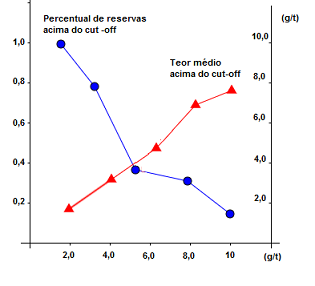
\includegraphics[scale=0.8]{curva_part.png}	
	\caption{Curva teor e tonelagem para um depósito mineral genérico. Na curva azul temos o valor da proporção do depósito para um dado cut-off, enquanto na curva vermelha temos o teor médio acima de um cut-off.}
	\label{curva_part}
\end{figure}

As curvas de teor e tonelagem são usuais em vários estágios da estimativa de depósitos. Durante a exploração mineral ela tem a importância de definir a caracterização inicial de recursos baseados nos dados de amostragem e garantir uma certa visualização de possíveis cenários para a mina. Nesta primeira iniciativa as estimativas ainda não se tornaram uma reserva devido a falta de um estudo de viabilidade. Durante a fase de operação, por exemplo, curvas de teor e tonelagem podem demonstrar possíveis cenários de mudança operacional, indicando as quantidades de material ainda presentes na mina que atendam as condições do beneficiamento. 


 Curvas de teor e tonelagem podem ser calculadas de diversas formas entre elas temos

\begin{itemize}
	\item Curvas derivadas de um histograma das amostras
	\item Curvas derivadas de uma distribuição de probabilidades contínua das amostras
	\item Curvas derivadas dos blocos estimados
	\item Curvas baseadas na variância de dispersão dos blocos estimados
\end{itemize}

\subsection{Curvas de teor e tonelagem derivadas de histogramas das amostras} \label{teor_t1}

Como dito no capítulo 1, as estimativas não podem aumentar ou criar informações acerca do depósito mineral. Tomando esse pressuposto é possível que histogramas desagrupados de amostras possam conter informação necessária para construir curvas de teor e tonelagem representativas, caso o procedimento de amostragem seja coerente. Ao realizar um histograma acumulado podemos encontrar o valor da proporção acima do teor de corte dado por \eqref{propor_tc}

\begin{equation}\label{propor_tc}
     P_{V\geq t_{c}} = 1-P_{V = t_{c}}
\end{equation}

Em que $P_{V = t_{c}}$ é a proporção para um dado teor de corte no histograma acumulado.  

Neste caso apenas os valores da classe estarão disponíveis para a inserção no gráfico. Quanto maior for o número de classes do histograma acumulado, maior será o número de pontos a serem plotados. Entre os valores das classes é possível realizar algum tipo de interpolação, lembrando que a curva é negativa definida, sempre diminuindo com o aumento do teor de corte. Técnicas como polinômios de Hermite são uma forma ideal de se aproximar estas curvas a partir dos dados dos histogramas. 

Para o cálculo da média dos valores acima do teor de corte determinado pode-se realizar no histograma a média dos valores das classes pelas suas proporções acima do limite estabelecido. Neste caso teremos um número de pontos também definido pelo número de classes  do histograma. A média é neste caso uma função positiva definida, técnicas de interpolação também podem ser utilizadas para se aproximar os valores entre classes. 

\subsection{Curvas de teor e tonelagem a partir de distribuição de probabilidades continuas das amostras}

Outra forma adequada de se calcular as curvas de teor e tonelagem a partir de amostras é considerando um ajuste de uma função de densidade de probabilidade para estas. No entanto, isso somente é possível de se fazer quando existe uma distribuição conhecida para o conjunto de dados analisados. Muitas vezes o padrão de proporções das amostras pode apresentar um comportamento não descrito pelas funções mais comuns de densidade de probabilidade.

\subsection{Curvas de teor e tonelagem baseadas na dispersão dos blocos estimados} \label{ref2}

Para estudos de viabilidade podemos criar uma curva de teor e tonelagem baseada na dispersão do bloco no volume do depósito. Dessa forma modificamos o histograma das amostras no suporte para o suporte da unidade seletiva de lavra. Utilizando a técnica de transformação afim podemos criar a curva de teor e tonelagem como descrito na seção \eqref{teor_t1}.

\subsection{Curvas de teor e tonelagem baseadas na estimativa dos blocos}

Ao contrário do procedimento relatado em \eqref{ref2} as curvas de teor e tonelagem obtidas pela estimativa dos blocos não necessitam de uma mudança de suporte para qualificar as unidades seletivas de lavra. Neste caso ela causa uma suavização nas curvas de teor e tonelagem fazendo com que os teores mais baixos tenham maiores proporções e os teores mais altos menores proporções. O gráfico \eqref{suav} demonstra a relação das curvas de cut-off para a proporção da jazida acima destes. 


\begin{figure}[H]
	\centering
	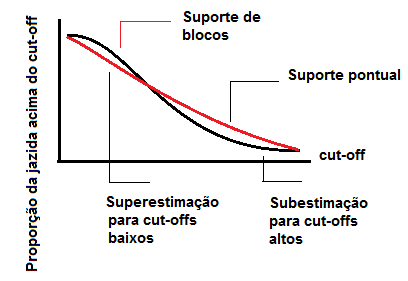
\includegraphics[scale=0.8]{suavizacao.png}	
	\caption{Demonstração da suavização da curva teor e tonelagem por mudança de suporte. Valores de cut-off mais baixos recebem maiores proporções, enquanto valores de cut-offs mais altos recebem maiores proporções}
	\label{suav}
\end{figure} 
 
 \subsection{Erros associados à determinação da curva de teor-tonelagem}
 
 Pequenos erros nas curvas de teor e tonelagem do depósito mineral podem causar grandes variações no retorno do investimento da mineração. Melhores protocolos de amostragem e estimativas mais confiáveis são uma alternativa para se reduzir estas variações. No caso de curvas realizadas a partir de histogramas ou de blocos estimados, o método de interpolação pode interferir na definição da curva. As curvas de teor e tonelagem são sempre enviesadas. Essa diferença dos valores reais e estimados pode ser reduzida com a mudança de suporte. Curvas realizadas com blocos estimados são sempre preferíveis à curvas realizadas de valores pontuais. 
  
